\section{Complete \lgname Syntax and Semantics}

\newcommand{\pgm}{\mathit{Program}}
\newcommand{\im}{\mathit{Module^+}}
\newcommand{\db}{\mathit{DeclBlock}}
\newcommand{\defs}{\mathit{Defs}}
\newcommand{\init}{\mathit{Init}}
\newcommand{\evnts}{\mathit{Event^+}}
\newcommand{\evnt}{\mathit{Event}}
\newcommand{\fdefs}{\mathit{FuncDef}}
\newcommand{\adefs}{\mathit{AdtDef}}
\newcommand{\args}{\mathit{Arg}^+}
\newcommand{\mterm}[1]{\mbox{ \textbf{#1} }}
\newcommand{\stmts}{\mathit{Stmt}^+}
\newcommand{\stmt}{\mathit{Stmt}}
\newcommand{\asgn}{\mathit{Assign}}
\newcommand{\cndnl}{\mathit{Ite}}
\newcommand{\floop}{\mathit{Loop}}
\newcommand{\fncall}{\mathit{FnCall}}
\newcommand{\atmc}{\mathit{Atomic}}
\newcommand{\decls}{\mathit{Decl}^+}
\newcommand{\decl}{\mathit{Decl}}
\newcommand{\var}{\mathit{Var}}
\newcommand{\val}{\mathit{Val}}
\newcommand{\type}{\mathit{Type}}
\newcommand{\awd}{\mathit{AWDecls}}
\newcommand{\ard}{\mathit{ARDecls}}
\newcommand{\ld}{\mathit{LocDecls}}
\newcommand{\cnd}{\mathit{Cond}}
\newcommand{\params}{\mathit{Param}^+}
\newcommand{\param}{\mathit{Param}}
\newcommand{\aports}{\mathit{APorts}}
\newcommand{\sports}{\mathit{SPorts}}
\newcommand{\expr}{\mathit{Expr}}
\newcommand{\aexpr}{\mathit{AExpr}}
\newcommand{\bexpr}{\mathit{BExpr}}
\newcommand{\id}{\left\langle\mathit{identifier}\right\rangle}
\newcommand{\aval}{\mathit{AVal}}
\newcommand{\bval}{\mathit{BVal}}
\newcommand{\ret}{\mathit{Return}}
\begin{figure*} \begin{mdframed}
\scriptsize
\begin{align*}
\begin{split}
\pgm &::= \defs\ [\im]\ \db\ [\init]\ \evnts\  \\\\
\defs &::= [\fdefs^+]\ [\adefs^+]\\
\fdefs &::= \mterm{def}\mterm{fun} \id ( \params ):\ \stmts\\  
\adefs &::= \mterm{def}\mterm{adt} \id :\ \decls\\
\param &:: \type\ \id \\\\
\mathit{Module} &::= \mterm{using}\mterm{module}\id : \sports\ \aports\\
\sports &::= \mterm{sensors}:\decls \\ 
\aports &::= \mterm{actuators}:\decls\\\\
\decl &:: \type\ \id \mid \type\ \id \ \mterm{=} \val \\
\type &::= \mterm{int}\mid \mterm{float}\mid\mterm{bool}\mid \mterm{pos}\mid \mathit{adt} \\ &\ \mid \type [\mathit{Int}]\mid \mterm{List}\left\langle\type\right\rangle \mid \mterm{Queue}\left\langle\type\right\rangle\\\\
\db &::= \awd\ \ard\ \ld\\
\awd &::= \mterm{allwrite}:\ \decls\\ 
\ard &::= \mterm{allread}:\ \decls\\ 
\ld &::= \mterm{local}:\ \decls\\\\
\init &::= \mterm{init}:\ \stmts\\
\evnt &::= \id: \mterm{pre}\ [\mterm{urgent}]\ (\cnd)\mterm{;}\mterm{eff}:\ \stmts\\
\end{split}\begin{split}
\expr &::= \aexpr | \bexpr \\
\aexpr &::= \aexpr\ \mathit{AOp}\ \aexpr\\  
&\mid \expr \mterm{++} \mid \mterm{-} \aexpr \mid \var \mid \aval \\
\mathit{AOp} &::= +\mid-\mid*\mid / \\ 
\bexpr &::=  \expr\ \mathit{RelOp}\ \expr | \expr\ \mathit{COp}\ \expr\\
&\mid \mterm{not} \expr \mid \var\mid \bval\\
\mathit{RelOp} &::=  \geq \mid \leq \mid \geq \mid == \mid > \mid < \mid \neq\\ 
\mathit{COp} &::=  \mterm{and} \mid \mterm{or} \\\\ 
\stmt &::= \asgn \mid \fncall\mid\atmc  \\ 
      & \mid\cndnl\mid \floop \mid \ret \\
\asgn &::= \var\ \mterm{=}\  \expr \\
\cndnl &::= \mterm{if} \bexpr\ \stmts \ [\mterm{else} \stmts]\\
\fncall &::= \id ([\aexpr\mid\bexpr]^+) \\
\atmc &::= \mterm{atomic}: \stmts\\
\floop &::= \mterm{For} \id \mterm{in} \aexpr : \stmts\\
\ret &::= \mterm{return} \expr \mid \mterm{return} \\\\
\var &::= \id \mid \id [\expr] \\ &\mid \id \mterm{.} \id \\
\val &::= \aval \mid \bval \\
\aval &::= \mathit{Int} \mid \mathit{Float}  \\
\bval &::= \mathit{Bool} 
\end{split}
\end{align*}\end{mdframed}
\caption{$\lgname$ program syntax.}
\label{fig:syntax}
\end{figure*}





\section{Code and Figures}
\chiao{Appendix should not be included for PLDI and should be provided separately as supplementary materials.
We just put figures and code here for now to count the pages.}


\subsection{Distributed Task Allocation}


\begin{figure}[h!]
    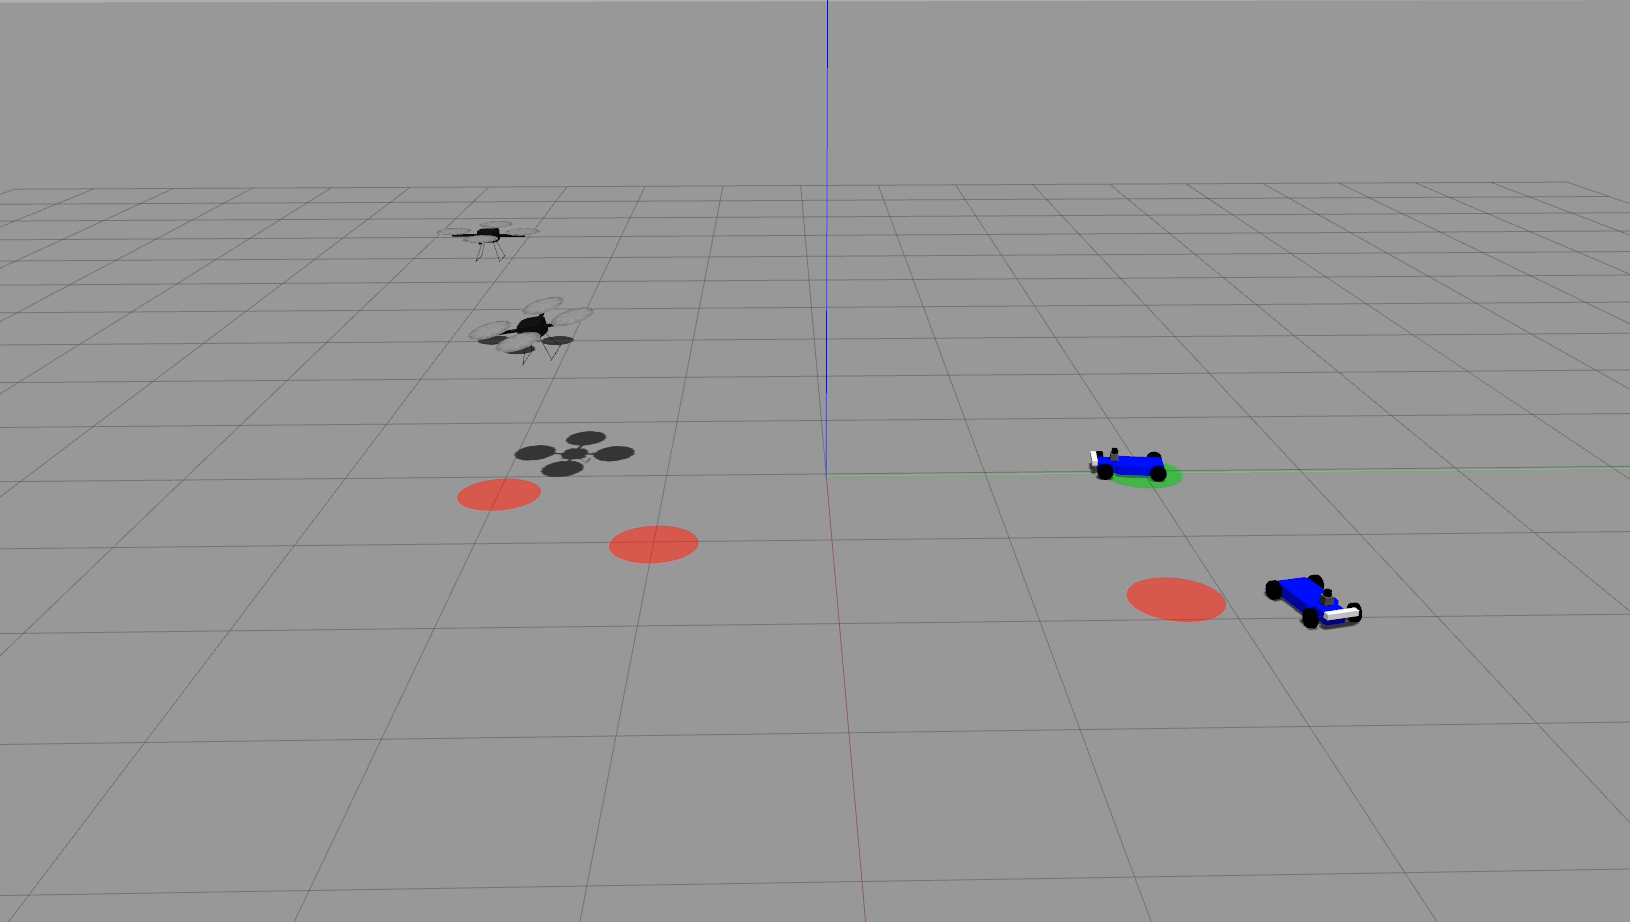
\includegraphics[width=\columnwidth]{figs/taskalloc_w_marker.png}

    \caption{Screenshot in the simulation of Distributed Task Allocation}
\end{figure}

\begin{figure*}[t]
    \two{0.4}{0.6}
    {
    \lstinputlisting[language=NumKoord, lastline=17]{code/taskalloc.tex}
    }
    {
    \lstinputlisting[language=NumKoord, firstline=18, firstnumber=18]{code/taskalloc.tex}
    }

    \caption{Distributed Task Allocation}
\end{figure*}


\subsection{Distributed Mapping Problem}
\sayan{
    Informally, the problem requires a set of robots to collaboratively mark the position of static \emph{obstacles} within a given area $D$, which any robot should avoid while moving in $D$.The key difference between distributed SLAM and this application is that we assume that the robots know their \emph{global coordinates} within the area of deployment. They are only attempting to map the static obstacles within this area. We currently assume that the only sensors available for sensing obstacles are LIDAR based, and the robots are constrained to move in a 2-D space.
}

\subsection{\dmap Application}

\reffig{flowmap1} shows a simple idea for solving the mapping problem problem for each robot, and \reffig{mapapp} shows our solution to $\dmap$ written using $\lgname$, a high level language with native support for multi-robot systems designed to interact with a physical environment. The design of solution to the mapping problem in \reffig{flowmap1} captures an occupancy map of the 2D space in a variable $\gmap$. \reffig{flowmap}. The variable $\lmap$ is a local mapping constructed by each robot $i$ using sensors, and information from other robots shared via $\gmap$. The robot first updates its $\lmap$ from $\gmap$, which stores the currently computed occupancy map \emph{by all robots}.  The robot then picks a new point in the grid known to be unoccupied in its $\lmap$ and follows a path ($\mathit{Motion.Path}$) moving only over grid rectangles known to be unoccupied by its $\lmap$. While the robot hasn't reached the target rectangle, it keeps updating its $\lmap$ with sensed data (occupied and unoccupied grid points). When it reaches the target, it updates the $\gmap$ with new data from its $\lmap$.


\begin{figure}[!htbp]
    \centering
    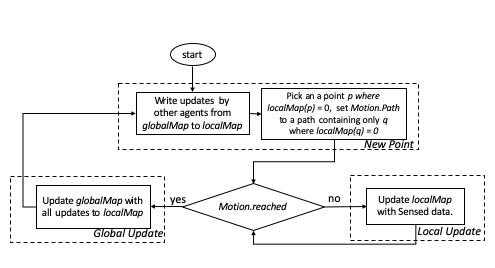
\includegraphics[width=\linewidth]{figs/map_flowchart.png}
    \caption{Flowchart for a simple solution to 2D distributed mapping problem\vspace{-2mm}}
    \label{fig:flowmap1}
\end{figure}

 An \emph{allwrite} variable is a shared variable which all robots can read from and write to. The shared \emph{allwrite} variable $\gmap$ is used to construct a shared map of obstacles within the domain $D$, and has type $\mathit{GridMap}$, which is a 2-D array representing a grid over $D$. The \emph{local} variable $\lmap$ represents each robot's \emph{local} knowledge of the domain $D$, and has the same type as $D$. A robot executing the \emph{NewPoint} event, first updates a \emph{local variable} $\lmap$ from the shared variable $\gmap$, using a combination operator $\oplus$, described in more detail in \refsect{prelims}. $\lgname$ allows the user to use library functions, like the $\mathit{findPath}$ function, which uses a path planner to find a path to a point while avoiding a set of \emph{obstacles}. The point is picked using the $\mathit{pickFrontierPos}$ function which is a user defined function implemented in $\lgname$. The details of the path planner, and how the point is picked are discussed in and \refsect{prelims} \refsect{experiments}.

In $\dmap$, there are two modules \emph{Motion} and \emph{Lidar} which provide interfaces to different sensors and actuators on the robot. The $\mathit{Lidar.ldata}$ sensor module is used to read the LIDAR scan of the actual robot. In the \emph{NewPoint} event, the controller driving the robot directs it along a path set at the actuator port $\mathit{Motion.path}$. The sensor port $\mathit{Motion.psn}$ gives the position of the robot (in a fixed coordinate system) and $\mathit{Motion.reached}$ indicates whether the controller is active or inactive.

The $\lgname$ program corresponding to this solution has three \emph{events}: \emph{NewPoint, LUpdate, GUpdate}. Each robot in the system runs an instance of the \emph{same} program. At runtime, the $\lgname$ program executes within the runtime system of a single robot, or a collection of programs execute on different robots. The $\lgname$ language semantics ensures that the execution of the program in the distributed system occurs in \emph{rounds} of duration $\delta$. In each round, each robot executes the statements in the effect(\textbf{eff}) of at most one \emph{enabled} event : an event whose precondition(\textbf(pre)) is satisfied. If no event is enabled, the robot does nothing. Before the next round of execution, the robot may continue to interact with the physical environment as directed by its controllers. The $\lgname$ semantics imposes a synchronous model of execution for $\lgname$ programs for multi-robot systems and its implementation in CyPhyHouse toolchain ensures that this schedule is maintained by the multi-robot system executing the $\lgname$ program, despite potentially imprecise synchronization of local clocks.

\begin{figure}[!htbp]
    \noindent
    \begin{center}
        \lstdefinelanguage{dmap}[]{NumKoord}{
            morekeywords=[2]{
                Grid, GridMap,
                Scan,
            }
        }
        \two{0.33}{0.62}
        {\lstinputlisting[language=dmap,firstline=1,lastline=22]{code/mapapp.tex}}
        {\lstinputlisting[language=dmap,firstline=23,firstnumber=23]{code/mapapp.tex}}
    \end{center}

    \caption{$\lgname$ code for robot $i$ for the 2D distributed mapping application.}
    \label{fig:mapapp}
\end{figure}

In the design of the $\dmap$ application, we employ the use of \emph{sampled} sensors, which is essentially a sequence of timestamped sensor readings between rounds. The \emph{LUpdate} event can occur while each robot is traversing a path and hasn't reached the final destination, during which the robot uses a sampled sensor reading of the positions $\mathit{Motion.trace}$, of type $\mathit{PosStamped}[]$, which denotes an array of timestamped positions; and a sampled sensor reading of LIDAR scans $\mathit{Lidar.ldata}$ of type $\mathit{ScanStamped}$, which denotes an array of timestamped LIDAR scans. These sampled sensor readings are then synchronized to associate a LIDAR scan with a position.

Mutual exclusion is an essential feature required in a distributed system with shared variables. The robot updates the shared variable $\gmap$ in the event \emph{GUpdate} using the value of its $\lmap$, which may have been updated with newly detected obstacles